\begin{justifying}
        
    \subsection*{(c)\textit{ Independencia de la trayectoria}}
    \noindent Mientras que el resultado de algunos procesos depende fundamentalmente de la
    trayectoria precisa en el espacio de estados, otros son {\textit{independientes de la trayectoria}} o casi
    lo son. Un caso particular de gran interés en todos los campos de investigación, desde la física
    hasta la sociología, es el de la equifinalidad, o mismo estado final. El concepto preciso
    es elucidado por

    \bigskip

    \noindent DEFINICIÓN 5.19: Dos cambios seriales son {\textit{equifinales}} si y solo si sus estados finales son
    los mismos.

    Se ha afirmado que la equifinalidad demuestra la finalidad o la orientación hacia un objetivo, ya que parece como si el sistema en cuestión —por ejemplo, un organismo— se esforzara por alcanzar un objetivo determinado por todos los medios a su alcance. Sin embargo, la equifinalidad no es una prueba de teleología a menos que se pueda demostrar la existencia de un propósito, ya que los procesos equifinales son comunes entre las cosas físicas. Por
    ejemplo, todos los sistemas termodinámicos cerrados se acercan a un estado de equilibrio.

    {\textit{Ejemplo}} Sea el valor instantáneo de una propiedad {\textit{F}} dado por una
    de las siguientes funciones en $\mathbb{R}^+$:

    \smallskip

    \begin{figure}[h!]
    \centering
    
    % --- COLUMNA IZQUIERDA (Imagen) ---
    \begin{minipage}{0.5\textwidth}
        \centering
        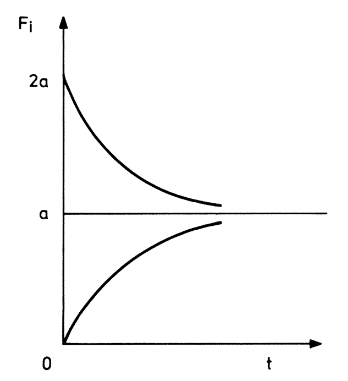
\includegraphics[width=0.95\textwidth]{img/Figura5-11.png}
    \end{minipage}%
    % --- COLUMNA DERECHA (Fórmulas) ---
    \begin{minipage}{0.45\textwidth}
        \vspace{1.5cm} 
        \begin{align*}
            F_1(t) &= a(1+e^{-kt}) \\
            F_2(t) &= a \\
            F_3(t) &= a(1-e^{-kt}) \\[1em]
            \text{con } & a, k \in R^+.
        \end{align*}
    \end{minipage}

    \vspace{10pt} % Un pequeño espacio vertical entre la imagen/fórmulas y el texto
    
    
    \parbox{\textwidth}{
        \centering
        \scriptsize 
        \text{Fig. 5.11.} Tres formas diferentes de alcanzar el mismo estado final o valor asintótico
        
        $X_{\infty} = a$ partiendo de $a$, avanzando hacia él o declinando hacia él.
    }
    
    \end{figure}

    \newpage

    \subsection*{(d)\textit{ Memoria}}
    \noindent Supongamos que el estado de una cosa depende no solo de un parámetro $t$ (la fase
    del proceso), sino también de algún estado o estados anteriores. 
    En este caso, se dice que la cosa tiene {\textit{memoria}} de algunos de sus estados pasados, 
    o que sufre un proceso {\textit{hereditario}}. Así, el estado elástico de una pieza
    de acero, el estado magnético de un imán y el estado genético de un organismo 
    dependen todos de sus historias previas. En varios casos, esa dependencia puede expresarse mediante una fórmula del tipo

    \[
        F(t) = \int_0^t F(\tau - t) \cdot M(\tau) \cdot \mathrm{d}\tau,
    \]

    \noindent donde $M$ es la función de memoria. (El proceso no tiene memoria si es $M$ = $\delta$,
    o la delta de Dirac).

    El concepto general se aclara mediante

    \medskip

    \noindent DEFINICIÓN 5.20 Sea $\mathbb{F}$ una función de estado y $S(x)$ el espacio de estados correspondiente,
    para una cosa $x$ relativa a un cierto marco de referencia. Además,
    llámese a $t \in T$ el parámetro de estado, donde $T$ es un conjunto dirigido. 
    Entonces $x$ experimenta un proceso {\textit{hereditario}} si y solo si cada uno de sus estados $\mathbb{F}(t) \in S(x)$ es un funcional 
    de algunos otros estados $\mathbb{F}(\tau)$ con $\tau<(t)$.

    Hay dos tipos importantes de procesos hereditarios: ($a$) la
    memoria se mantiene bastante intacta durante todo el proceso, y ($b$ ) 
    la memoria se desvanece hasta desaparecer prácticamente después de un cierto tiempo llamado {\textit{tiempo de relajación}}. 
    Los sistemas con componentes que interactúan débilmente, como
    los gases no ionizados y los imperios extendidos, tienen tiempos de relajación cortos. 
    Por otro lado, los organismos tienen tiempos de relajación genética y ontogenética largos. 
    Por ejemplo, la desnutrición y la privación de la socialidad en las primeras etapas de la vida de un mamífero son suficientes 
    por separado para perjudicar gravemente algunas de sus capacidades para la vida.

    \subsection*{(e)\textit{ Reversibilidad e irreversibilidad}}
    \noindent Algunos procesos, especialmente a nivel microfísico —y probablemente solo esos—, son reversibles; todos los macroprocesos conocidos son irreversibles.
    Esto último puede considerarse una generalización de un teorema demostrado en mecánica estadística. Un sistema se denomina {\textit{érgodico}} si finalmente explora todo su espacio de estados o, 
    más precisamente, si, cuando se deja inalterado (aislado), ocupa sucesivamente todos los estados compatibles con su energía total.

    \smallskip

    \noindent Hasta 1913, la mayoría de los autores afirmaban que, dado que las partículas individuales se mueven
    de forma reversible, toda colección de partículas debe tener la propiedad de reversibilidad y, además, debe ser ergódica. 
    Ese año, A. Rosenthal y M. Plancherel demostraron de forma independiente que, si el sistema satisface las ecuaciones canónicas (cap. 3, sec. 2.6), entonces no es ergódico. 
    Es decir, demostraron que no existen sistemas ergódicos (o totalmente reversibles) de la mecánica clásica. 
    Por lo tanto, incluso si el universo fuera un enorme agregado de partículas (que no lo es), no podría volver sobre todos sus pasos. 
    No existe el eterno retorno.

    Finalmente, observamos que en microfísica se asume que la mayoría de los procesos, aunque no todos, son {\textit{estocásticamente reversibles}}, 
    en el sentido de que la probabilidad de un proceso elemental y la de su inverso son iguales. Esto permite desviaciones momentáneas de la tendencia general, 
    es decir, eventos aislados en los que algunos estados se vuelven superpoblados o subpoblados. Sin embargo, ciertos microprocesos, en particular la radiactividad y, 
    en general, los procesos de transmutación, son irreversibles.

    Todo esto invita a

    \smallskip

    \noindent DEFINICIÓN 5.21 Sea $\pi(x) = \langle \mathbb{F}(t) \mid t \in T \rangle$ En un proceso serial en una cosa x.
    Además, sea $\bar{T}$ el mismo conjunto que $T$ dirigido en sentido opuesto (por ejemplo, $\langle \mathbb{R}, > \rangle$  en lugar de $\langle \mathbb{R}, < \rangle$. 
    Entonces $\pi(x)$ es reversible si y solo si $\bar{\pi}(x) = \langle \mathbb{F}(t) \mid t \in \bar{T} \rangle$ es tan posible (es decir, legal) como $\pi(x)$.

    Si tanto a $\pi(x)$ como a su inverso $\bar{\pi}(x)$ se les pueden asignar 
    probabilidades, se puede pensar en definir el \textit{grado de reversibilidad} 
    de un proceso como la razón de su probabilidad y la de su inverso, o 
    $r = \bar{p}/p$. Para un proceso totalmente reversible, $r=1$; para un 
    proceso bastante reversible, $0 \ll r < 1$; para un proceso casi irreversible, 
    $0 < r \ll 1$; y para un proceso totalmente irreversible, $r=0$. 
    Tal concepto podría ser útil en varios campos, particularmente en la 
    mecánica estadística.

    Es común declarar que un proceso es reversible solo en caso de que sus leyes 
    sean invariantes bajo la inversión del tiempo. Esto es un error, porque los 
    procesos dependen tanto de las circunstancias como de las leyes. Por ejemplo, 
    aunque las leyes básicas de la desintegración radioactiva (principalmente 
    las de Schrödinger) son $T$-invariantes, las condiciones de frontera son tales 
    que la probabilidad de que un fragmento de la desintegración reingrese al 
    núcleo se anula.

    Finalmente, nótese que, si bien todos los procesos reversibles son cíclicos, 
    lo contrario es falso. De hecho, la mayoría de los ciclos no son reversibles – 
    es decir, no dejan las cosas como estaban. Por ejemplo, el ciclo del agua y el 
    ciclo del nitrógeno en nuestro planeta no son reversibles, ya que están 
    acompañados por una degradación de la energía (aumento de la entropía).

    \subsection*{(f)\textit{ Proceso aleatorio}}
    \noindent Un tipo conspicuo de proceso en serie, y uno de gran interés filosófico, 
    es el de un proceso aleatorio. (Para una definición de aleatoriedad, 
    véase Cap. 4, Sec. 6.4.) Un proceso aleatorio o estocástico es aquel 
    que se describe por una función de estado que es una “variable” aleatoria, 
    es decir, una función cada uno de cuyos valores tiene una probabilidad 
    o densidad de probabilidad definida. En el caso más simple, los valores 
    $s_i$ de la función de estado $\mathbb{F}$ forman una secuencia discreta 
    $\langle s_i \mid i \in \mathbb{N} \rangle$, como los tiempos de llegada de 
    los clientes a un mostrador. En este caso, la función $f$ tal que 
    $f(s_i) = \mathrm{Pr}(\mathbb{F}(t) = s_i) = p_i$, donde $\mathrm{Pr}$ 
    es una medida de probabilidad y $p_i$ la probabilidad de que $x$ se encuentre 
    en el estado $s_i$, se denomina la \textit{distribución de probabilidad} 
    de $\mathbb{F}$. (Véase, por ejemplo, Feller, 1968, Cap. IX.)

    Muchas propiedades sustanciales, en todos los niveles, deben ser representadas 
    por ``variables'' aleatorias. Por lo tanto, cualquier proceso real ---en 
    contraste con un modelo idealizado del mismo--- es probable que tenga al menos 
    un aspecto aleatorio. Por consiguiente, en lugar de definir el concepto de 
    un proceso real (como es habitual en la bibliografía sobre procesos 
    estocásticos) preferimos adoptar

    \newpage

    \noindent DEFINICIÓN 5.22 Sea $\mathbb{F}$ $ = \langle F_1, F_2, \dots, F_n \rangle$ 
    una función de estado para una cosa $x$ que experimenta un cambio en serie 
    $\pi(x) = \langle \mathbb F(t) \mid t \in T \rangle$. Se dice que este proceso es 
    \textit{aleatorio en el i-ésimo aspecto} si y solo si la componente $F_i$ 
    de $\mathbb{F}$ es una variable aleatoria.

    \subsection*{(g)\textit{ Estabilidad}}
    \noindent Se dice que una cosa es estable si su punto representativo en el espacio de 
    estados permanece confinado dentro de una región ``pequeña''. Más 
    precisamente, podemos hacer

    \bigskip

    \noindent DEFINICIÓN 5.23 Sea $G_{\mathbb{L}}(x)$ el conjunto de transformaciones 
    lícitas del espacio de estados $S_{\mathbb{L}}(x)$ de una cosa $x$. Entonces $x$ es 
    \textit{estable en la región} $A \subset S_{\mathbb{L}}(x)$ si y solo si, para todo 
    $s \in S_{\mathbb{L}}(x)$, $g(s) \in A$ para todo $g$ en $G_{\mathbb{L}}(x)$.

    En otras palabras, una cosa está en un estado de \textit{equilibrio dinámico} 
    si todos los cambios que experimenta la llevan a un subconjunto fijo de su 
    espacio de estados. Si este subconjunto se reduce a un punto, entonces se 
    dice que la cosa está en \textit{equilibrio estático} o que no cambia en 
    absoluto. En otras palabras, una cosa $x$ está en equilibrio estático en un 
    estado $a \in S_{\mathbb{L}}(x)$ si y solo si $a$ es un punto fijo bajo cada 
    transformación del espacio de estados en sí mismo ---es decir, si $g(a) = a$ 
    para todo $g \in G_{\mathbb{L}}(x)$. En resumen, así como los subconjuntos fijos 
    del espacio de estados representan el equilibrio dinámico, los puntos fijos 
    representan los estados de equilibrio estático.

    Los estados de equilibrio estático solo pueden ser temporales. Por otro lado,
    el equilibrio dinámico puede ser duradero. La figura 5.12 muestra los estados de

    \newpage

    \begin{center}
        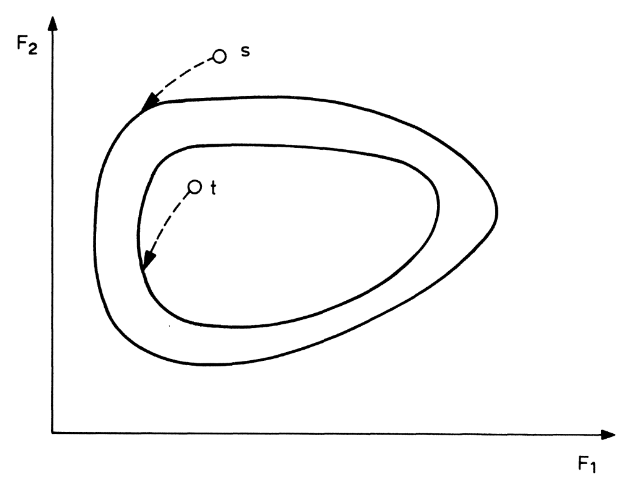
\includegraphics[width=0.8\textwidth]{img/Figura5-12.png}
        \\ \scriptsize Fig. 5.l2. Los equilibrios ecológicos son dinámicos. 
            Si una perturbación externa, como la agricultura o una sequía, envía el 
            punto representativo a $s$, o a $t$, el punto finalmente se mueve a una 
            órbita de equilibrio. (Véase, por ejemplo, Pielou (1969).)
    \end{center}

    \noindent equilibrio dinámico de un ecosistema que consiste en dos poblaciones en 
    competencia. Cada curva representa un proceso cíclico ---una oscilación 
    en el número de las poblaciones. Cada punto situado sobre una de las 
    curvas cerradas representa un estado estable del sistema. Si las poblaciones 
    son desplazadas ---por ejemplo, por alguna perturbación externa--- a valores 
    no muy lejanos del equilibrio, tienden a regresar espontáneamente a un 
    punto de equilibrio.

    Hasta aquí los tipos especiales de procesos. Apresurémonos a advertir que, 
    en nuestra opinión, ningún proceso real es de un tipo puro. Esto se debe a 
    que cualquier función de estado (realista) tiene una serie de componentes 
    de diferentes tipos ---algunos discretos, otros continuos, algunos aleatorios, 
    otros no aleatorios, y así sucesivamente. En otras palabras, llámese

    \[
        \pi_k(x) = \langle F_k(t) \mid t \in T \rangle, \quad \text{con } 1 < k \leq n
    \]

    \noindent la \textit{k-ésima componente} del proceso en serie representado por 
    $\pi(x)$ =$\langle \mathbb{F}(t) \mid t \in T \rangle$. Entonces $\pi(x)$ tendrá 
    al menos una componente continua, al menos una componente aleatoria, y así 
    sucesivamente. En resumen, los tipos de procesos puros

    \newpage

    \noindent son tipos ideales: los procesos reales son impuros. Dejamos la formulación
    exacta para la siguiente subsección.

    En primer lugar, nos centraremos en algunas generalidades que pueden formularse en términos bastante
    exactos.

    \subsection{Conceptos y principios generales}
    \noindent En la subsección anterior discutimos algunos tipos de procesos típicos. 
    En la presente trataremos los procesos en general, utilizando algunas ideas 
    obtenidas en el estudio de tipos de procesos especiales. De ese estudio se 
    desprende que un proceso puede ser considerado ya sea como una \textit{secuencia 
    de estados} o como una \textit{secuencia de eventos}. En el primer caso podemos 
    describir un proceso en una cosa $x$ con la única ayuda de una función de estado 
    $\mathbb{F}$ para ello: nuestra tarea se reduce a seguir los recorridos de la 
    punta de $\mathbb{F}$ ---una tarea enormemente facilitada al parametrizar los 
    estados $\mathbb{F}(t)$ en relación con los estados de un marco adecuado. Si, 
    por otro lado, interpretamos un proceso como una secuencia de eventos, entonces 
    se nos debe dar no solo $\mathbb{F}$ sino también todo el espacio de estados 
    $S_{\mathbb{L}}(x)$ abarcado por $\mathbb{F}$, así como la totalidad $G_{\mathbb{L}}(x)$ de 
    las transformaciones lícitas del espacio de estados en sí mismo. Solo esto 
    nos permite formar los eventos individuales $\langle s, s', g \rangle$ y, a 
    partir de ahí, todo el espacio de eventos $E_{\mathbb{L}}(x)$.

    Cada una de estas interpretaciones alternativas tiene sus ventajas y desventajas. 
    El enfoque de los estados sucesivos es matemáticamente más simple, aunque solo 
    sea porque el espacio de estados es $n$-dimensional mientras que el espacio 
    de eventos correspondiente es $2n$-dimensional. Por otro lado, el enfoque 
    de los eventos sucesivos, aunque matemáticamente más torpe, es filosóficamente 
    más perspicaz. Podemos usar cualquiera de los dos enfoques indistintamente y 
    así lo haremos. En la presente subsección discutiremos algunos principios 
    generales en términos de eventos, pero terminaremos introduciendo una noción 
    de historia basada en el enfoque de los estados sucesivos.

    Primero, las nociones generales del proceso:

    \bigskip

    \noindent DEFINICIÓN 5.24 Sea $E_g(x)$ el espacio de eventos de tipo 
    $g$ en la cosa $x$, para $g$ en el conjunto $G_{\mathbb{L}}(x)$ de transformaciones 
    lícitas del espacio de estados escogido para $x$, y sea $E(x)$ la unión de 
    todos los $E_g(x)$'s, es decir, el espacio total de eventos de $x$ 
    [Definición 5.9]. Además, sea $<$ la relación de precedencia [Definición 5.10]. 
    Entonces 
    
    (i) un \textit{proceso de tipo g} en la cosa $x$ es un conjunto 
    estrictamente parcialmente ordenado de eventos de clase $g$:

    \[
        \pi_g(x) = \langle E_g^*(x), < \rangle \quad \text{con } E_g^*(x) 
        \subseteq E_g(x) \subseteq E_\mathbb{L}(x);
    \]

    (ii) un proceso en x es un conjunto estrictamente parcialmente ordenado

    \[
        \pi(x) = \langle E^*(x), < \rangle \quad \text{con} \quad E^*(x) = 
        \bigcup_{g \in G_\mathbb{L}(x)} E_g^*(x).
    \]

    Dado que, de hecho, cada aspecto g está relacionado con algún otro aspecto,
    podemos suponer con seguridad que no hay procesos de un solo tipo, sino
    solo idealizaciones que destacan ahora una característica de lo que nos interesa,
    ahora otra. (Recuerde el final de la última subsección). Es decir, suponemos

    \bigskip

    \noindent POSTULADO 5.6 Todo proceso real tiene más de un aspecto.

    Y de la supuesta legalidad de las transformaciones en $G_{\mathbb{L}}(x)$se deduce
    que todo proceso que implique una cosa determinada satisface todas las leyes
    que posee esta última:

    \bigskip

    \noindent COROLARIO 5.9 Todos los procesos son legales.

    Tenga en cuenta que la legalidad se basa en procesos, es decir, en conjuntos de eventos intrínsecamente ordenados,
    y no en conjuntos de eventos arbitrarios. Estos últimos, especialmente si ocurren en cosas no relacionadas, o en cosas 
    con componentes débilmente acoplados,
    no son necesariamente legales, aunque se suponga que cada componente tiene una línea de comportamiento legal.
    Esto es el Este es el fundamento ontológico de la regla metodológica empleada tácitamente por
    los historiadores que se proponen descubrir tendencias históricas generales o incluso leyes,
    es decir, centrarse en procesos de un tipo definido que se producen en los sistemas sociales
    en lugar de limitarse a buscar series temporales, que están destinadas a ser
    erráticas o ilegales (véase Braudel, 1969).

    Recuerde, sin embargo, que el caos no es lo mismo que la aleatoriedad: mientras que el primero carece de ley, 
    el segundo posee leyes estocásticas (probabilísticas) como las de la mecánica cuántica y la genética. Por lo tanto, 
    adoptamos un axioma que emplea la Definición 5.22 de un proceso aleatorio en algún aspecto:
    
    \bigskip

    \noindent POSTULADO 5.7 Todo proceso es aleatorio en al menos un aspecto.

    Luego distinguimos dos miembros importantes de un proceso:

    \bigskip

    \noindent DEFINICIÓN 5.25 Sea $\pi(x) = \langle E^*(x), < \rangle$ 
    un proceso en una cosa $x$. Entonces

    (i) $\pi(x)$ \textit{comienza} en un evento $b \in E^*(x)$ si y solo 
    si $b$ es una cota inferior del conjunto $E^*(x)$ [es decir, si cualquier 
    otro miembro de $E^*(x)$ sigue a $b$];

    (ii) $\pi(x)$ \textit{termina} en un evento $e \in E^*(x)$ si y solo 
    si $e$ es una cota superior del conjunto $E^*(x)$ [es decir, si todos los 
    demás miembros de $E^*(x)$ preceden a $e$].

    \begin{center}
        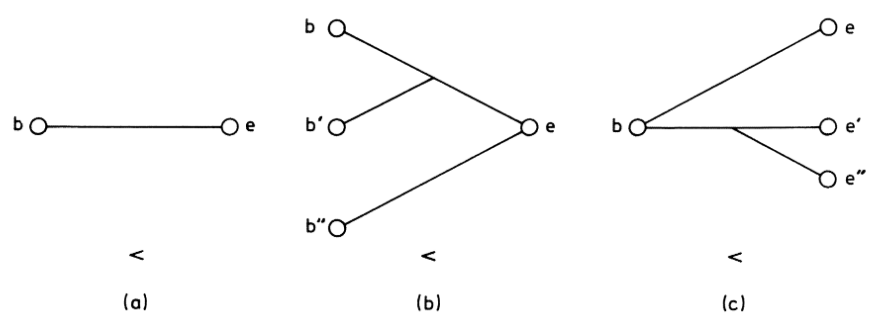
\includegraphics[width=0.8\textwidth]{img/Figura5-13.png}
        \\ \scriptsize Fig. 5.l3. Tres tipos de procesos en cuanto al inicio y el final. (a) Proceso en cadena o lineal. (b)
        Proceso convergente o ramificado. (c) Proceso divergente o ramificado.
    \end{center}

    Un proceso puede no tener un único inicio ni un único final: véase la figura 5.13.
    En otras palabras, puede haber múltiples inicios o múltiples finales. Suponemos 
    que cada proceso está limitado tanto por arriba como por abajo:

    \bigskip

    \noindent POSTULADO 5.8 Todo proceso tiene principio(s) y fin(es). 
    [Es decir, si $\pi(x)$ es un proceso que ocurre en una cosa $x$, entonces 
    $\pi(x)$ tiene al menos un principiante y al menos un punto final.]

    Esta hipótesis no implica que haya comienzos absolutos (es decir, procesos 
    que empiezan de la nada) y callejones sin salida (es decir, procesos que, 
    al terminar, no inician ningún otro proceso). De hecho, el postulado es compatible 
    tanto con una cosmología creacionista y escatológica como con la suposición de que 
    cada proceso en una cosa dada, aunque limitado tanto por abajo como por arriba, 
    está precedido y seguido por otros procesos, ya sea en la misma cosa o en otras cosas. 
    Adoptamos la última hipótesis porque es la que respalda la ciencia. Pero primero necesitamos

    \bigskip

    \noindent DEFINICIÓN 5.26 Sean $\pi(x)=\langle E^*(x), < \rangle$ y 
    $\pi'(x)=\langle E'^*(x), < \rangle$ dos procesos en una cosa $x$, tales que 
    $E^*(x) \cap E'^*(x) = \emptyset$. Entonces $\pi(x)$ \textit{precede} a 
    $\pi'(x)$ si y solo si cada evento en el primero precede a cada evento en el 
    segundo. Símbolo: $\pi(x) < \pi'(x)$.

    Estamos listos para

    \bigskip

    \noindent POSTULADO 5.9 Cada proceso está precedido y seguido por otros procesos. 
    Más precisamente, cada cosa $x$ tiene partes $y$ y $z$, no necesariamente diferentes de $x$, 
    cada una de ellas equipada con su propio espacio de eventos, de tal manera que.

    \[
        \pi(y) < \pi'(x) < \pi''(z).
    \]

    Dado que el mundo es la suma de todas las cosas, se deduce que

    \bigskip

    \noindent COROLARIO 5.10 El mundo no tiene principio ni fin.

    \textit{Observación 1} Al igual que muchos otros axiomas de nuestra ontología, el anterior
    es una especie de generalización de todo lo que sabemos. Un paradigma antiguo es,
    por supuesto, el proceso de nacimiento-crecimiento-desintegración final que experimenta todo metazoario. 
    Un paradigma más simple y moderno es el del fotón emitido por una estrella, que viaja a través del espacio interestelar y termina
    atrapado por una molécula o convirtiéndose en un par de electrones de cargas opuestas.
    \textit{Observación 2} En un momento dado, algunos cosmólogos que deseaban salvar la cosmología del estado 
    estacionario introdujeron la hipótesis \textit{ad hoc} de la creación espontánea de átomos de hidrógeno en el espacio vacío. 
    Esta conjetura no fue aceptada porque choca con las leyes de conservación (Bunge, 1962) y, en cualquier caso, 
    la teoría del estado estacionario, que intentaba salvar, fue finalmente refutada por las pruebas astronómicas.
    \textit{Observación 3} Corolario 5.10 Fue formulado por primera vez por los filósofos presocráticos y adoptado por Aristóteles. 
    Parecería contradecir la hipótesis del ``Big Bang'' sobre el ``origen'' del universo, hoy en día casi universalmente aceptada. 
    Sin embargo, esta conjetura cosmológica —que explica la expansión del universo— no ilustra la creación \textit{ex nihilo}, ya que presupone que
    el universo existía —en un estado altamente condensado— antes de que comenzara la expansión. Tampoco la antigua hipótesis 
    de la ``muerte térmica'' (hoy en día casi olvidada) ilustra la aniquilación absoluta: lo único que afirma es el fin del movimiento macrofísico 
    una vez que un sistema cerrado ha alcanzado el equilibrio térmico.

    Hasta aquí nuestros conceptos y principios generales sobre el proceso. Adoptemos ahora el enfoque de los estados sucesivos e introduzcamos una 
    noción clave más que resultará indispensable en la secuela, a saber, la de historia.

    Recuérdese que los estados de una cosa $x$ pueden ser coordenados en relación 
    con los estados $t \in S(f)$ de un marco de referencia $f$, definiendo la 
    función de estado como una aplicación de $S(f)$ en $S(x)$, y construyendo 
    $S(f)$ como una cuadrícula cuatridimensional que conceptualiza un marco de 
    referencia físico (Sec. 2.5). A medida que el estado de referencia $t$ se 
    ``mueve'', también lo hace la punta $\mathbb{F}(t)$ de la función de estado de la cosa. 
    Esto invita

    \bigskip

    \noindent DEFINICIÓN 5.27 Sea $\mathbb{F}$ una función de estado para 
    una cosa $x$ relativa a un marco de referencia $f$ con estados $t \in S(f)$, 
    y sea este último coordenado por una cierta función $k: \mathbb{R}^4 \to S(f)$. 
    Entonces la \textit{historia de $x$ relativa a $f$} es el conjunto de pares 
    ordenados

    \[
        h(x) = \{\langle t, \mathbb{F}(t) \rangle \mid t \in S(f)\}.
    \]

    Esta es una elucidación del concepto de línea de vida, línea de comportamiento 
    o trayectoria. La historia de una cosa se considera como la sucesión de sus 
    estados pero, en lugar de ser representada por una línea en el espacio de 
    estados $n$-dimensional abarcado por $\mathbb{F}$, se representa como una 
    curva en el espacio ($n+4$)-dimensional $\mathbb{R}^4 \times S_\mathbb{L}(x)$. 
    (La dimensionalidad de este espacio puede reducirse en 3 si estamos interesados 
    solo en la coordenada temporal, es decir, si $t$ se interpreta como un instante 
    de tiempo en lugar de como un punto en la región del espaciotiempo adjunta al 
    marco dado.)

    La definición anterior abarca los conceptos más habituales de historia empleados 
    en las ciencias. En particular, encaja con el concepto de historia que aparece en 
    una de las teorías más fundamentales de la física, a saber, la mecánica cuántica. 
    De hecho, en esta teoría, el operador de evolución de una cosa se define como

    \[
        S(t_0, t) = \exp\left(-\frac{i}{\hbar}\int_{t_0}^{t} du H\right),
    \]

    \newpage

    \noindent donde H es el hamiltoniano de la cosa. La historia de este último es entonces
    \[
        h(x) = \{\langle \langle t, S(t_0, t) \rangle \psi(t_0) \rangle \mid u \in [t_0, t] \ \& \ \psi \in \text{espacio de Hilbert de } x\}.
    \]

    El amplio concepto de historia adoptado anteriormente puede desconcertar e 
    incluso enfurecer a aquellos estudiosos de las humanidades que todavía 
    consideran al hombre como algo sobrenatural. Hasta aproximadamente mediados 
    del siglo XIX se había asumido tácitamente que toda la historia es historia 
    humana. Así, Hegel, a pesar de todo su dinamismo, negaba que la naturaleza 
    tuviera una historia. Esa visión cambió con los descubrimientos revolucionarios 
    en geología y biología, hasta el punto de que Engels declaró que cada ciencia 
    es la historia de algo (Engels, 1878). Desde entonces, se suele dar por sentado 
    que \textit{toda cosa tiene una historia} ---es decir, que, para toda cosa $x$, 
    $h(x)$ es más grande que un singulete.

    Apliquemos ahora el concepto de historia a una caracterización de las nociones 
    de acción e interacción.

\end{justifying}